\section{Pruning}
\label{app:Pruning}

\subsection{Asimov fit}
\label{app:PruningInAsimov}
Figures \ref{fig:Pruning_Asimov_Hp1000_Contained80_DL1r_70} to \ref{fig:Pruning_Asimov_Hp3000_Contained80_DL1r_70} show the pruning applied in the systematic uncertainties for the Asimov fits for all the $H^{+}$ mass fits.

%%% Pruning result for H+(1000)
\begin{figure}[H]
  \centering
  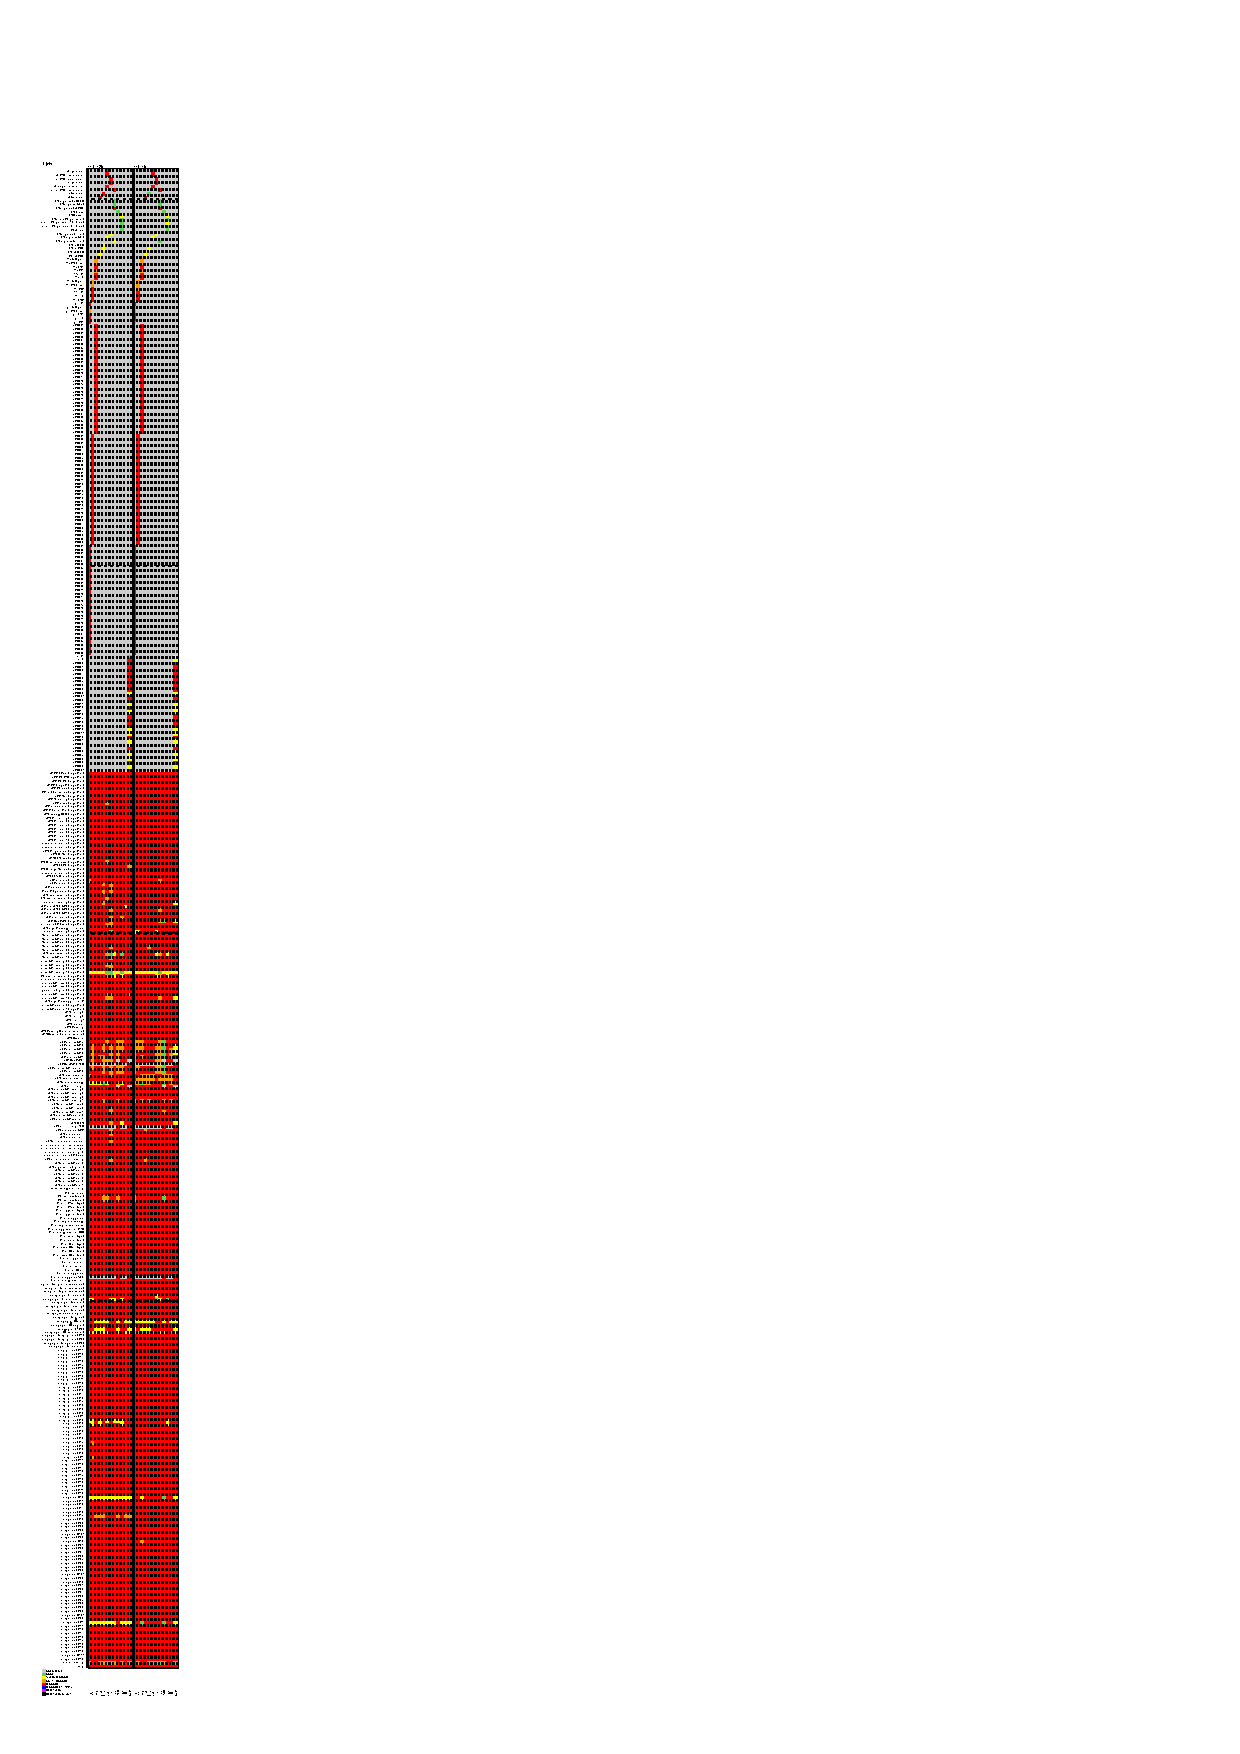
\includegraphics[keepaspectratio, scale=0.85]{images/Pruning/Pruning_Asimov_Hp1000_Contained80_DL1r_70.pdf}
  \caption{Pruned systematic uncertainties in the 1000 GeV $H^{+}$ mass Asimov fits}
  \label{fig:Pruning_Asimov_Hp1000_Contained80_DL1r_70}
\end{figure}

%%% Pruning result for H+(1200)
\begin{figure}[H]
  \centering
  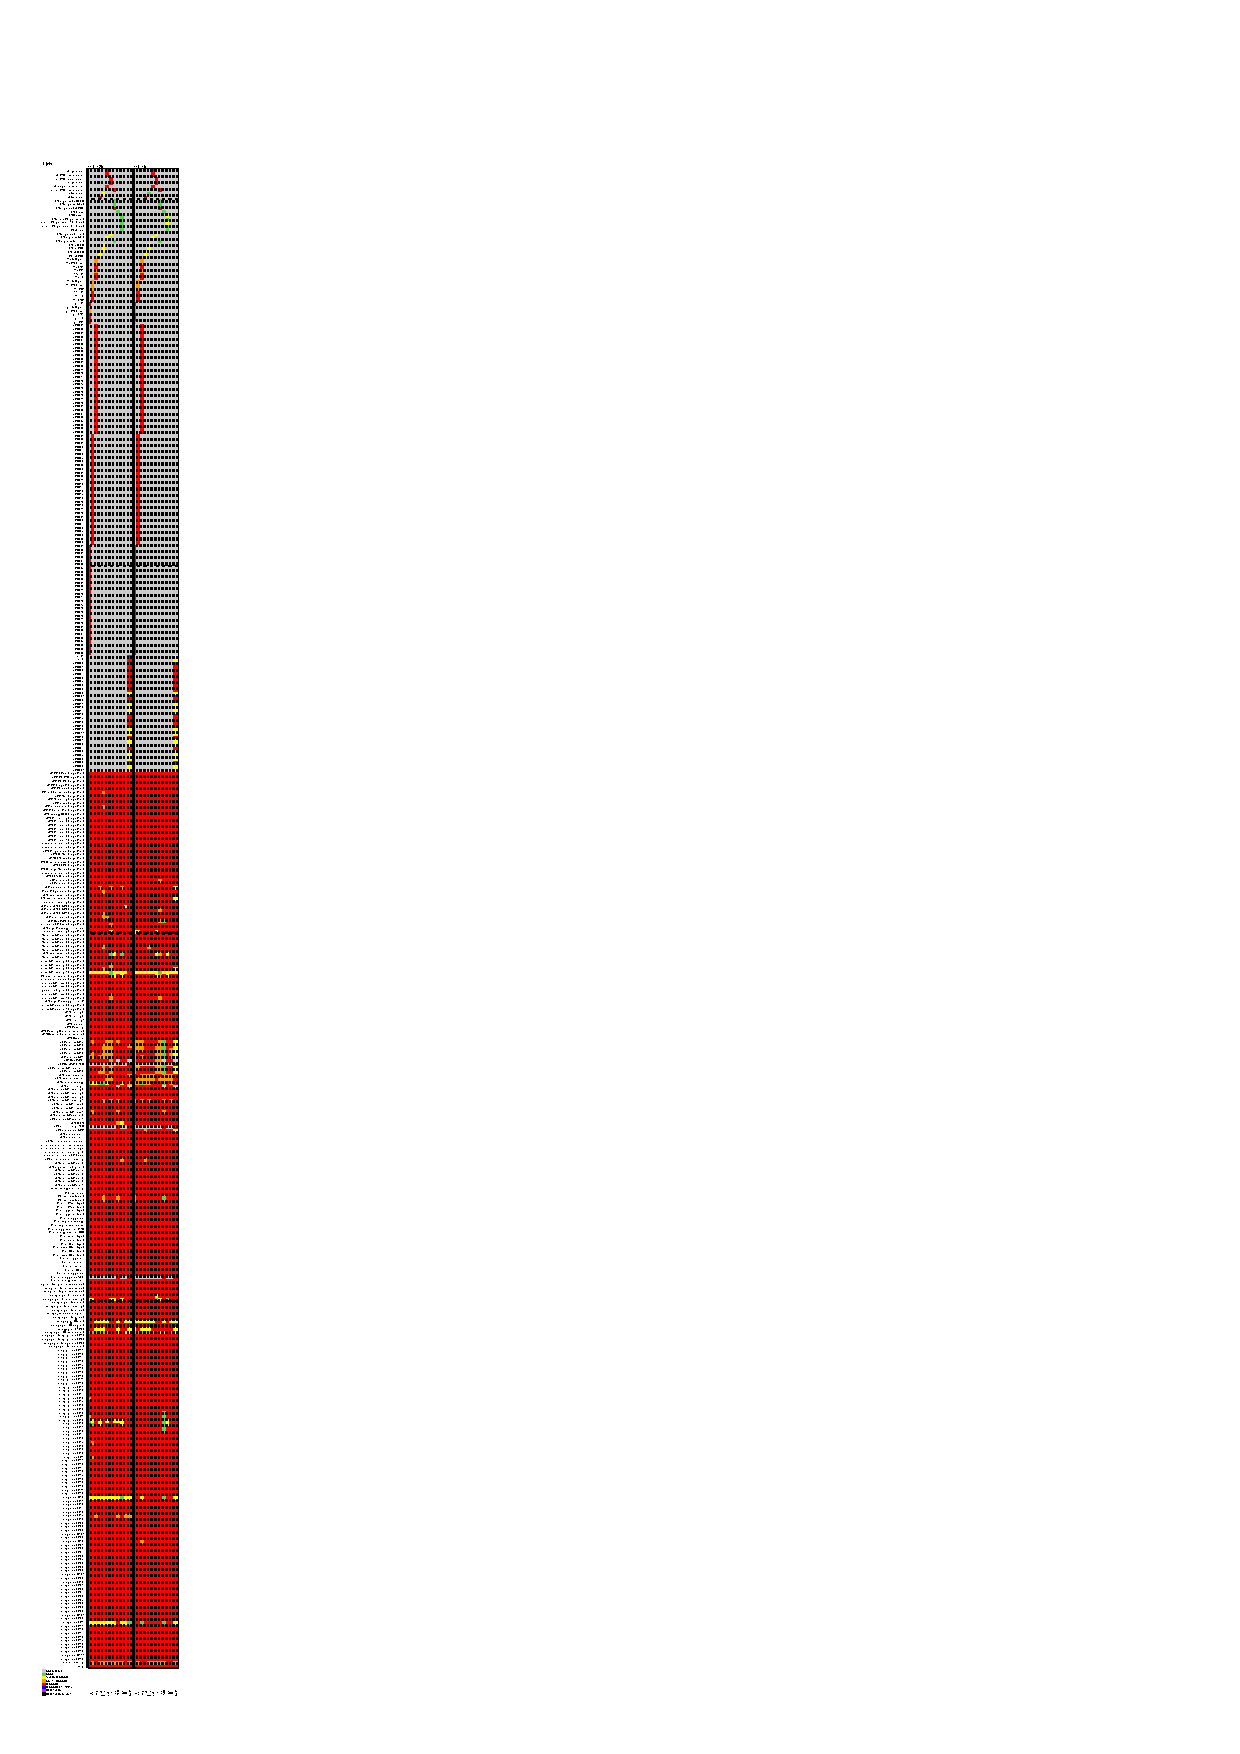
\includegraphics[keepaspectratio, scale=0.85]{images/Pruning/Pruning_Asimov_Hp1200_Contained80_DL1r_70.pdf}
  \caption{Pruned systematic uncertainties in the 1200 GeV $H^{+}$ mass Asimov fits}
  \label{fig:Pruning_Asimov_Hp1200_Contained80_DL1r_70}
\end{figure}

%%% Pruning result for H+(1400)
\begin{figure}[H]
  \centering
  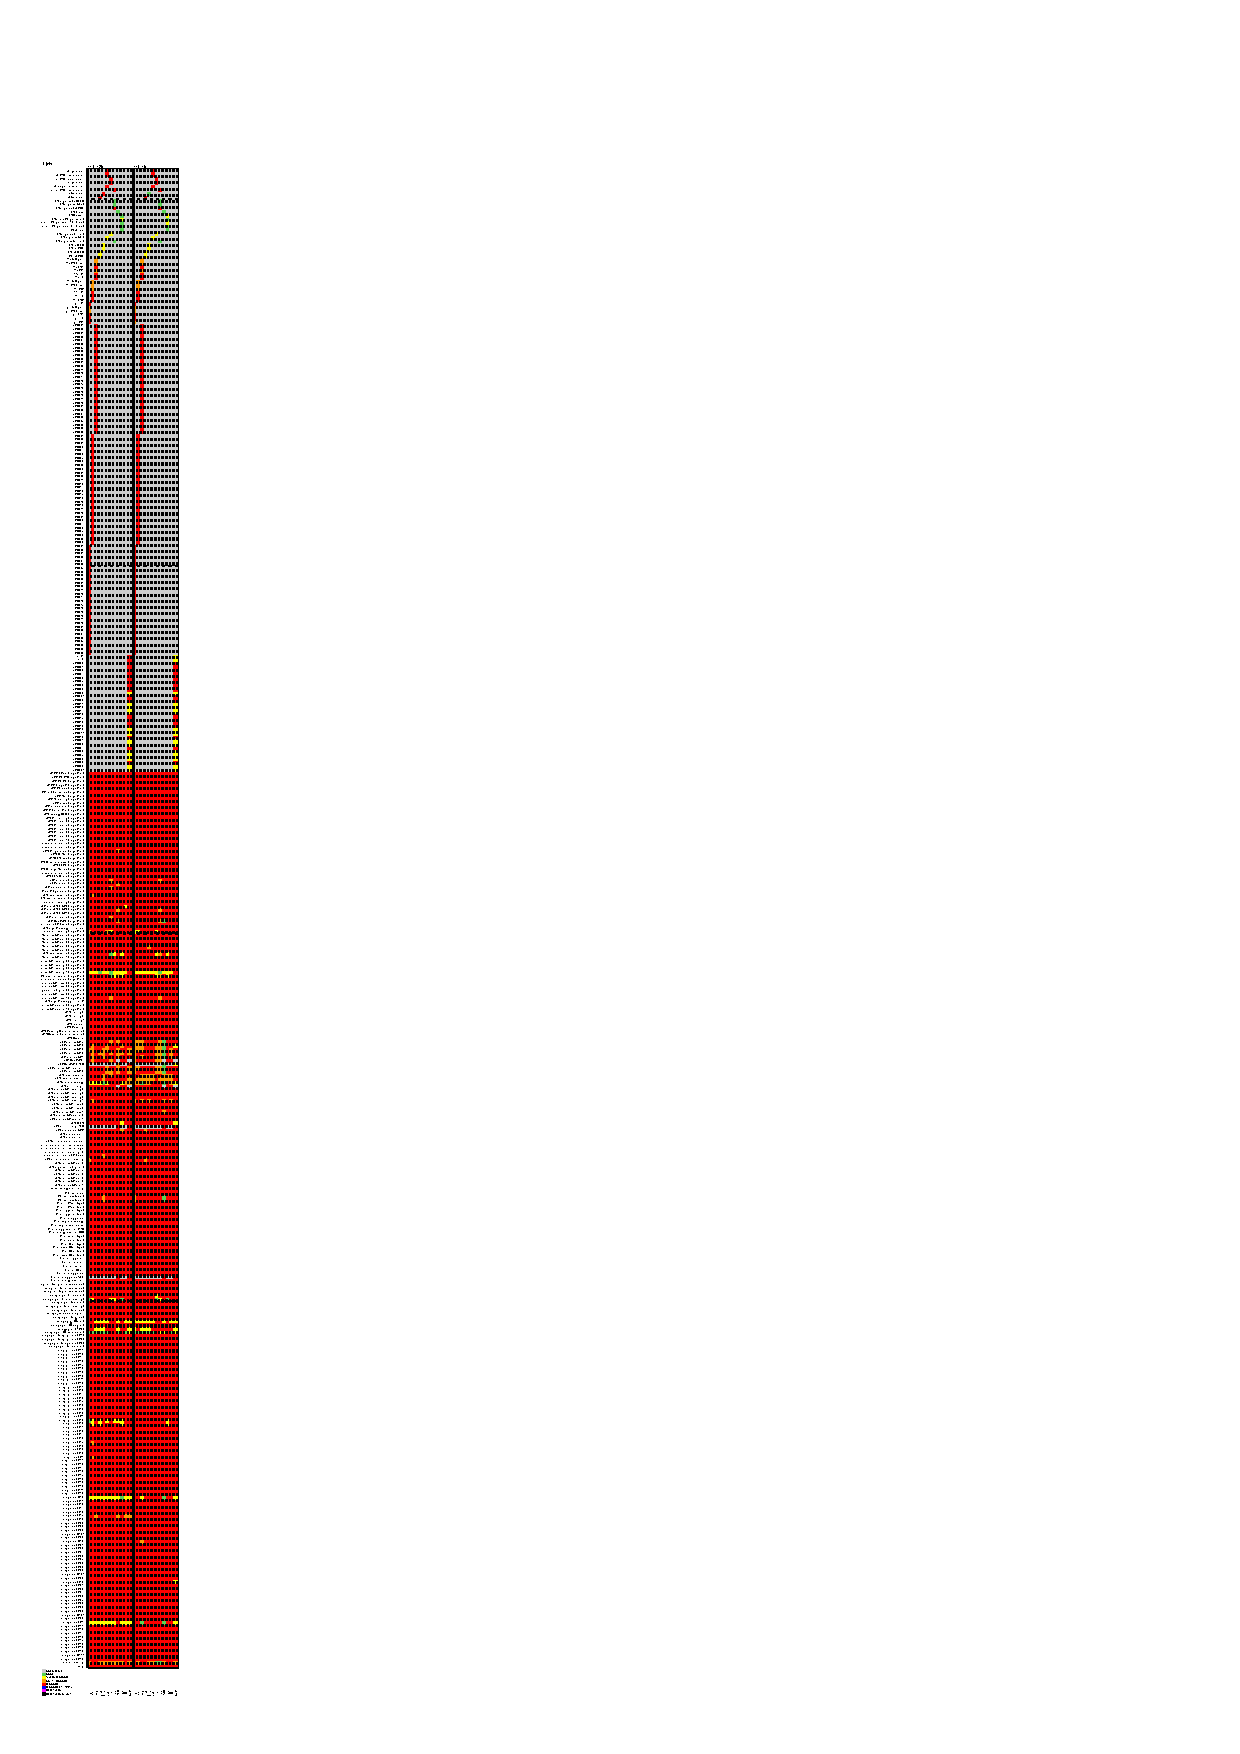
\includegraphics[keepaspectratio, scale=0.85]{images/Pruning/Pruning_Asimov_Hp1400_Contained80_DL1r_70.pdf}
  \caption{Pruned systematic uncertainties in the 1400 GeV $H^{+}$ mass Asimov fits}
  \label{fig:Pruning_Asimov_Hp1400_Contained80_DL1r_70}
\end{figure}

%%% Pruning result for H+(1600)
\begin{figure}[H]
  \centering
  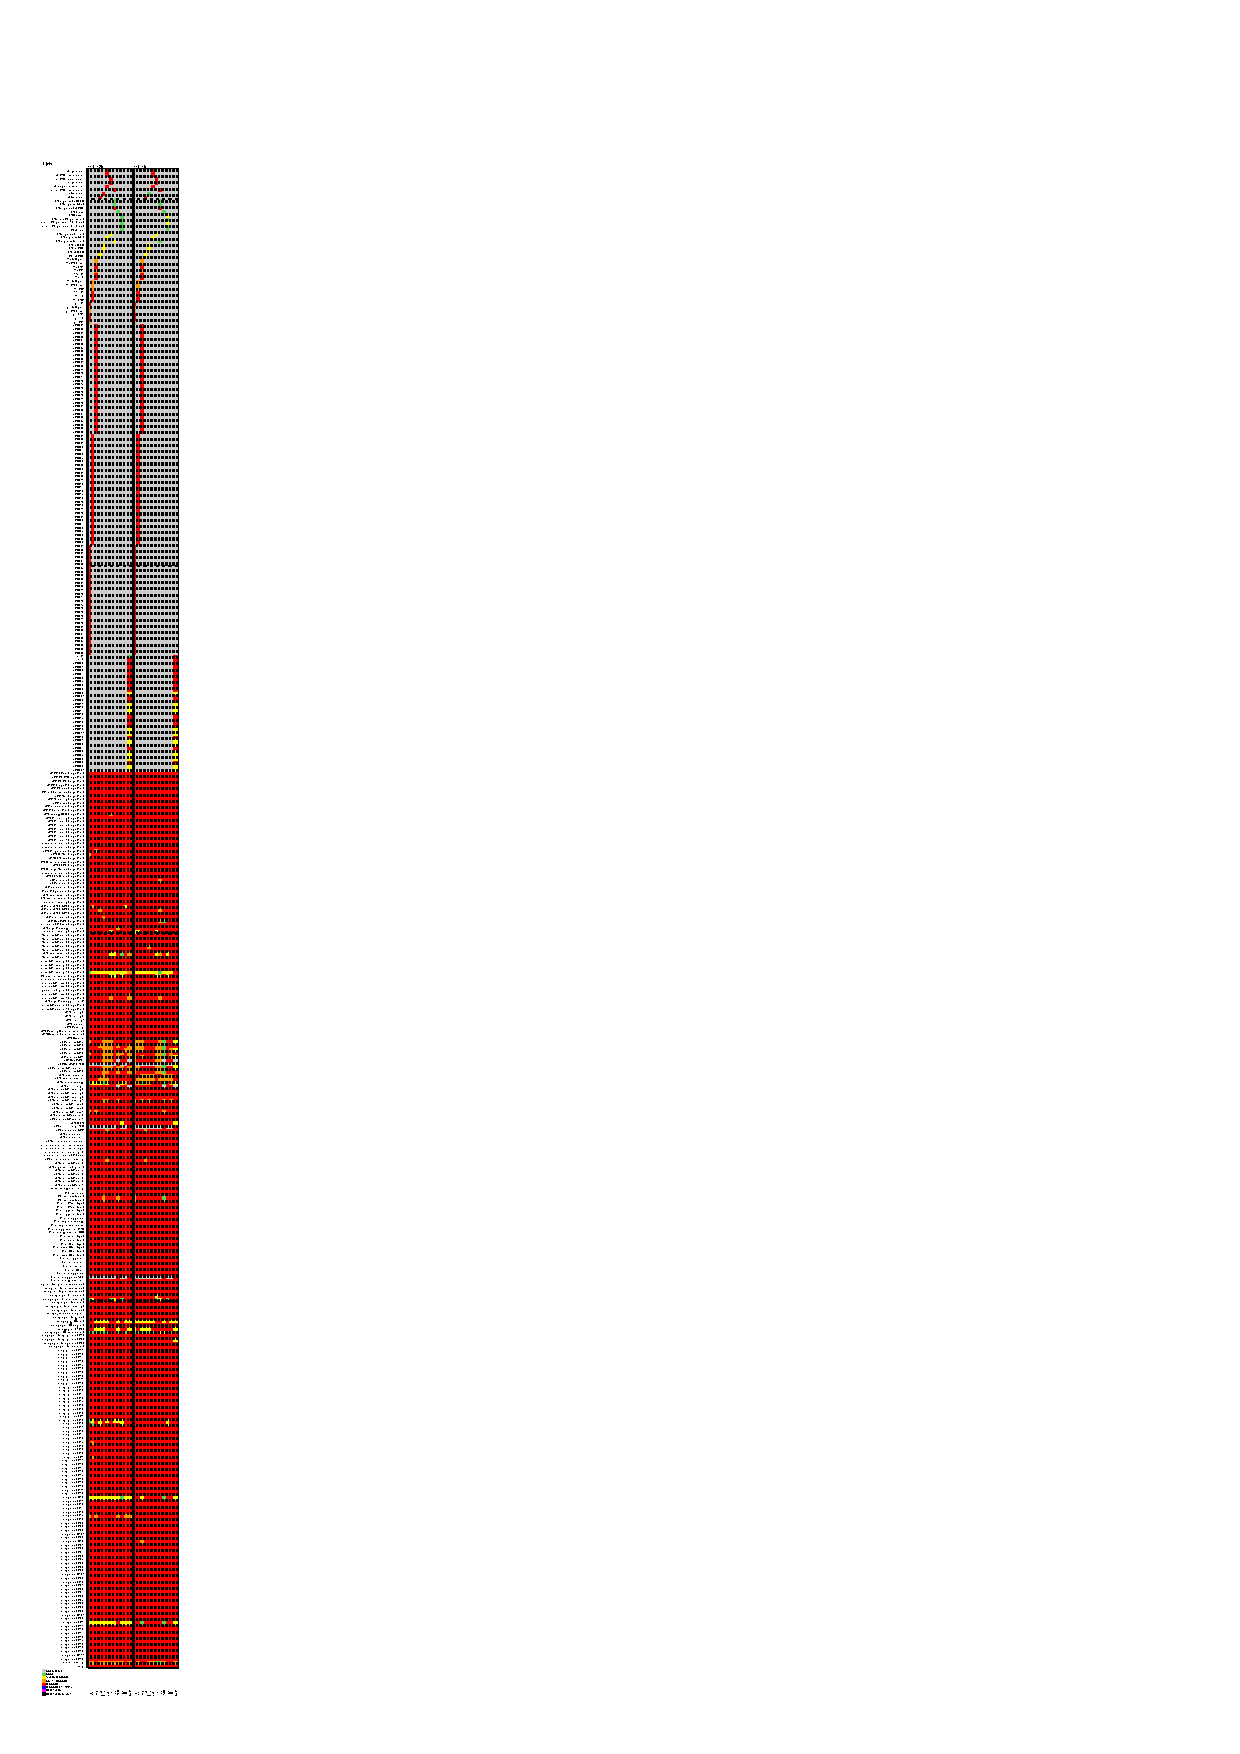
\includegraphics[keepaspectratio, scale=0.85]{images/Pruning/Pruning_Asimov_Hp1600_Contained80_DL1r_70.pdf}
  \caption{Pruned systematic uncertainties in the 1600 GeV $H^{+}$ mass Asimov fits}
  \label{fig:Pruning_Asimov_Hp1600_Contained80_DL1r_70}
\end{figure}

%%% Pruning result for H+(2000)
\begin{figure}[H]
  \centering
  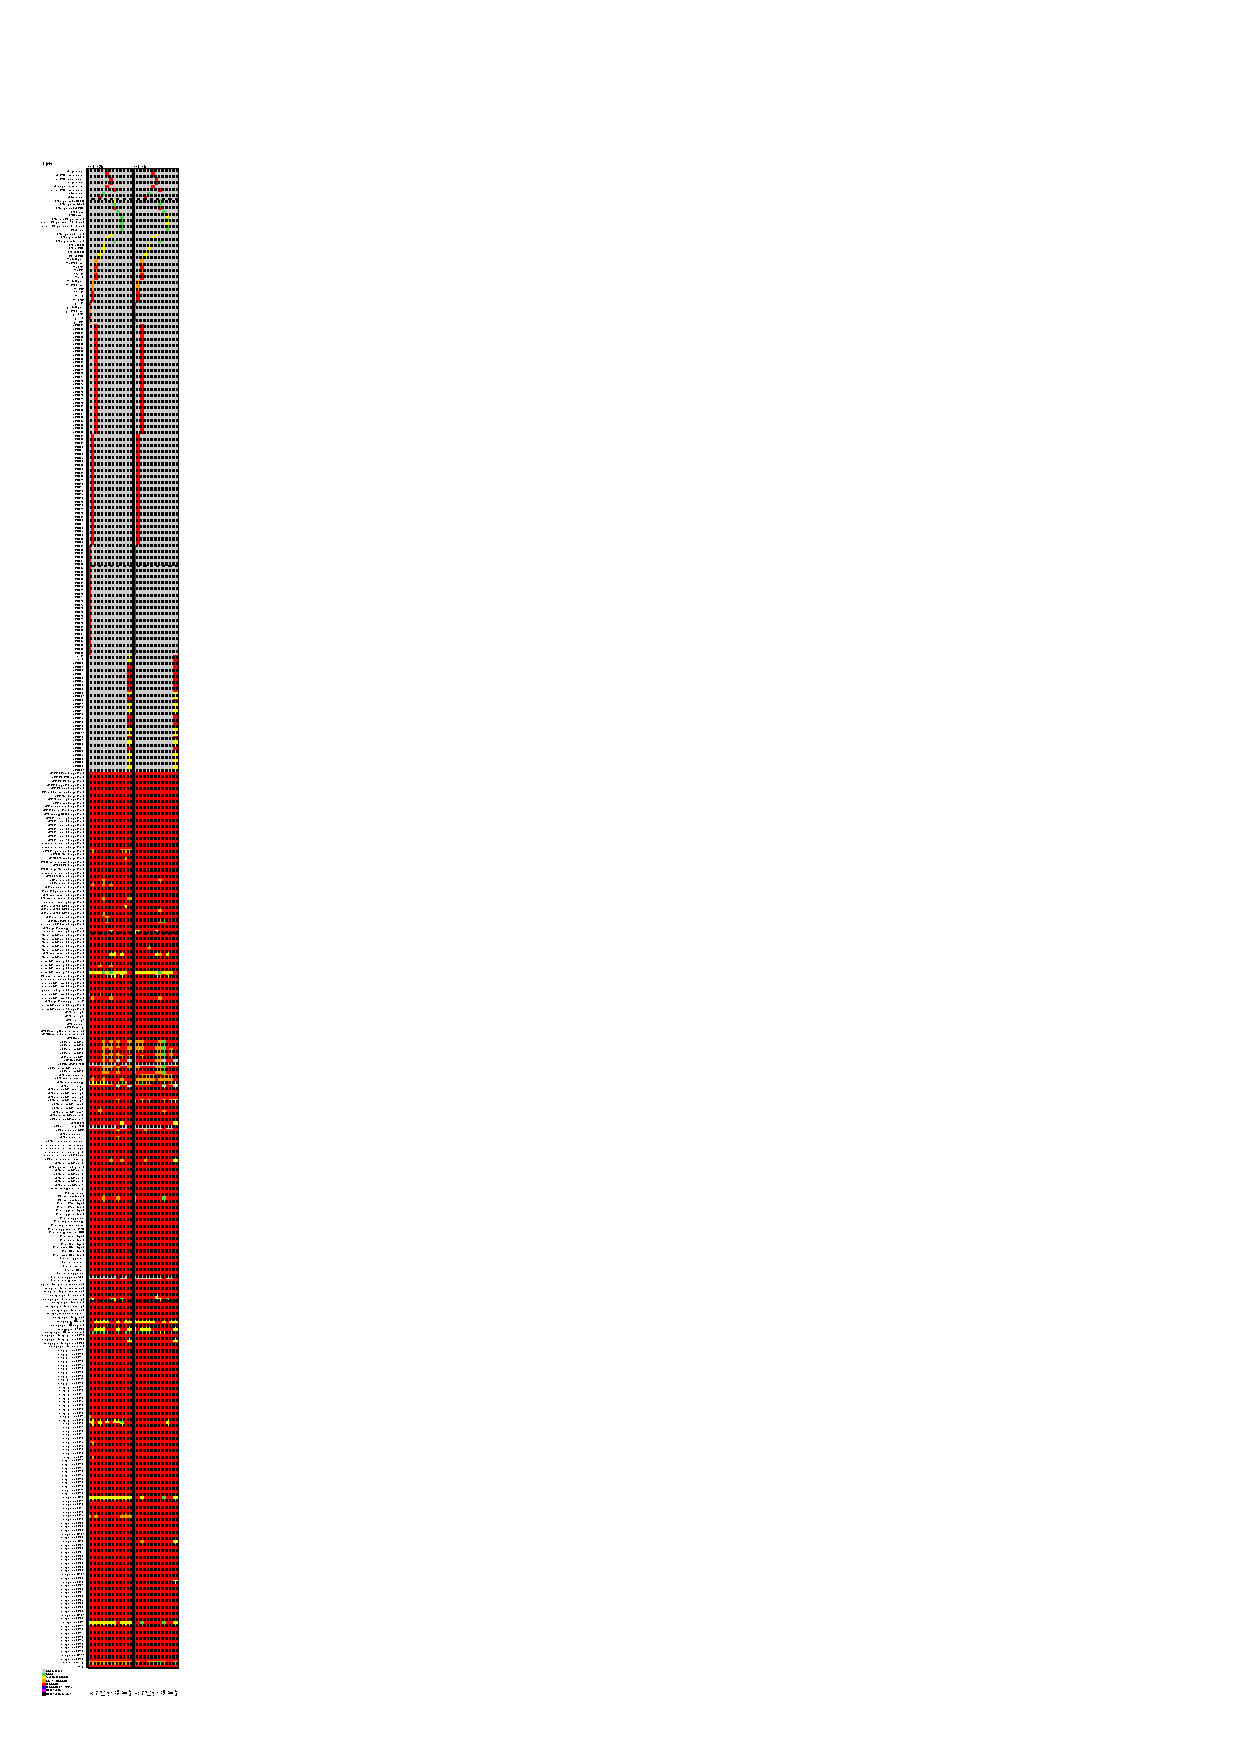
\includegraphics[keepaspectratio, scale=0.85]{images/Pruning/Pruning_Asimov_Hp2000_Contained80_DL1r_70.pdf}
  \caption{Pruned systematic uncertainties in the 2000 GeV $H^{+}$ mass Asimov fits}
  \label{fig:Pruning_Asimov_Hp2000_Contained80_DL1r_70}
\end{figure}

%%% Pruning result for H+(2500)
\begin{figure}[H]
  \centering
  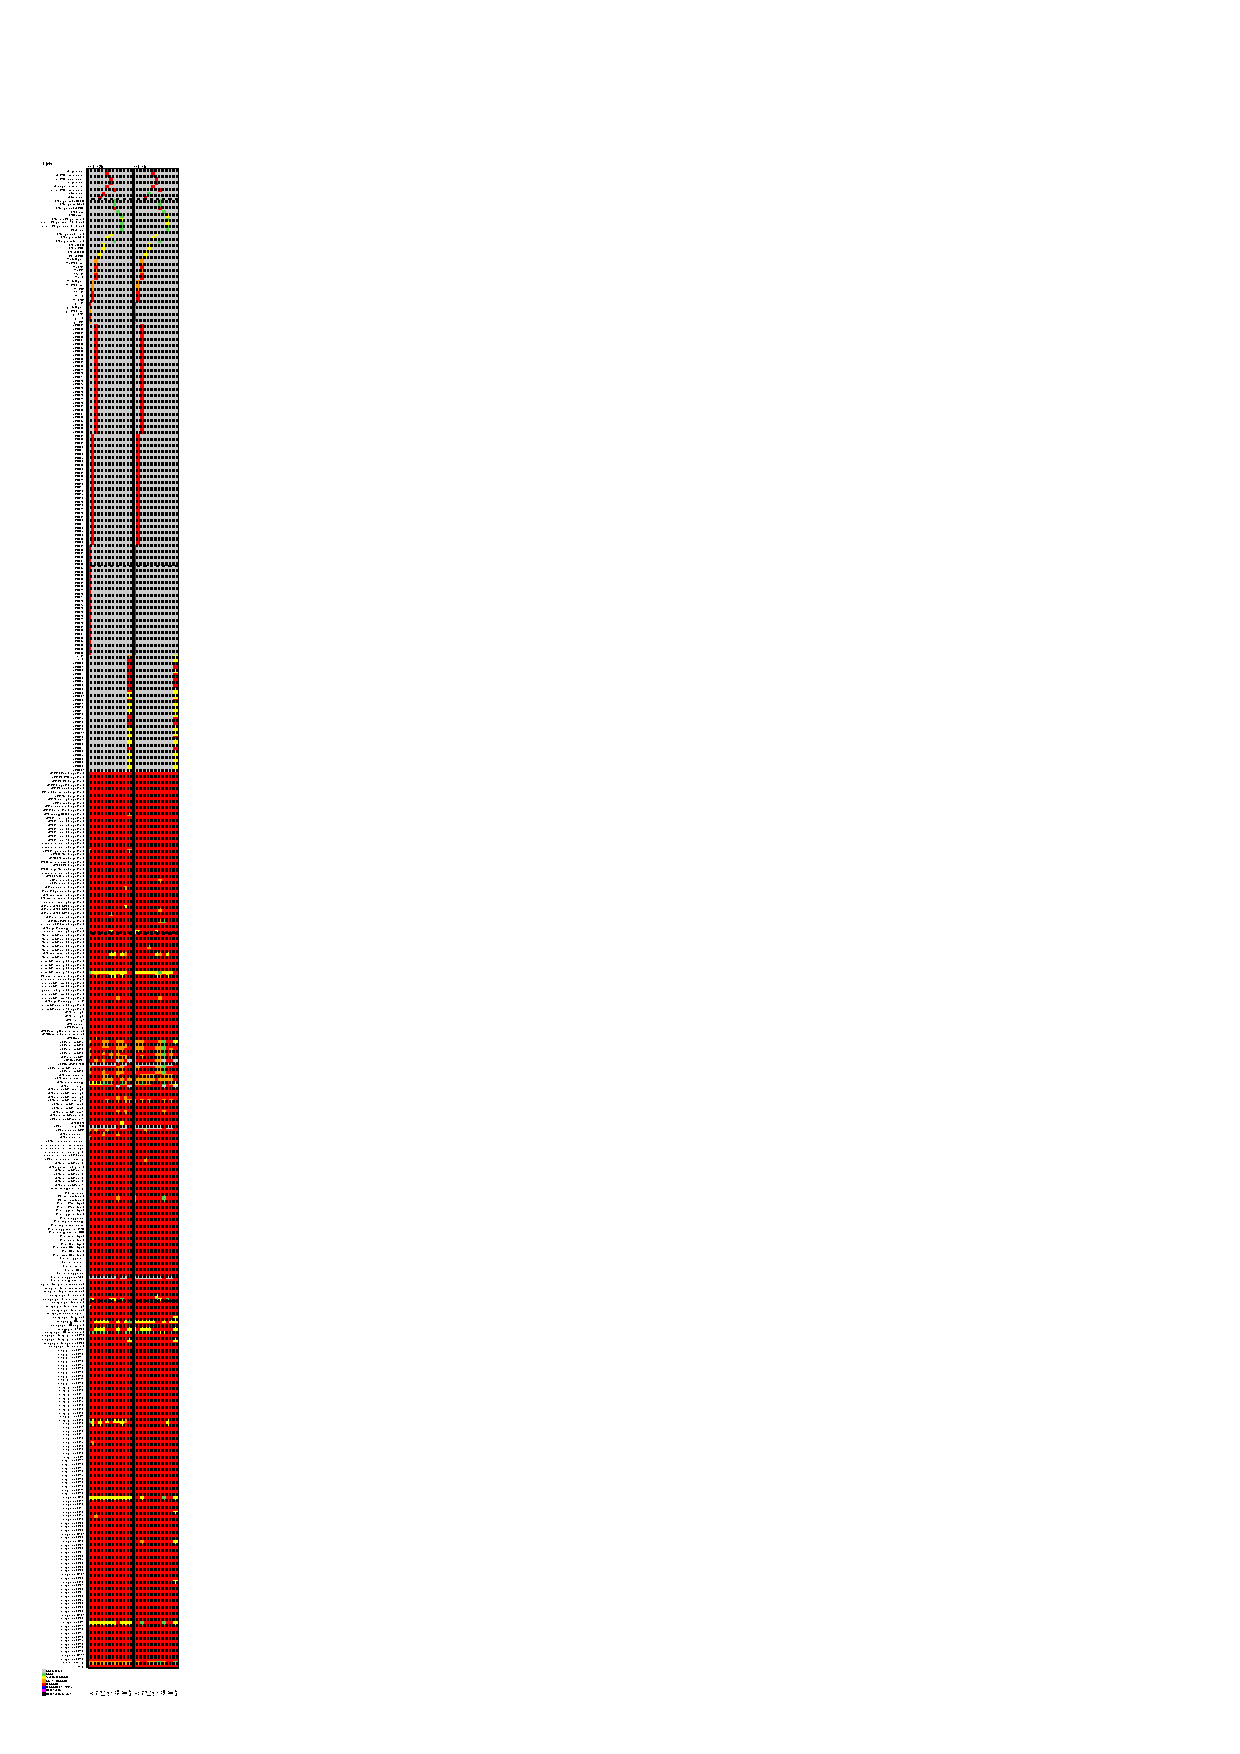
\includegraphics[keepaspectratio, scale=0.85]{images/Pruning/Pruning_Asimov_Hp2500_Contained80_DL1r_70.pdf}
  \caption{Pruned systematic uncertainties in the 2500 GeV $H^{+}$ mass Asimov fits}
  \label{fig:Pruning_Asimov_Hp2500_Contained80_DL1r_70}
\end{figure}

%%% Pruning result for H+(3000)
\begin{figure}[H]
  \centering
  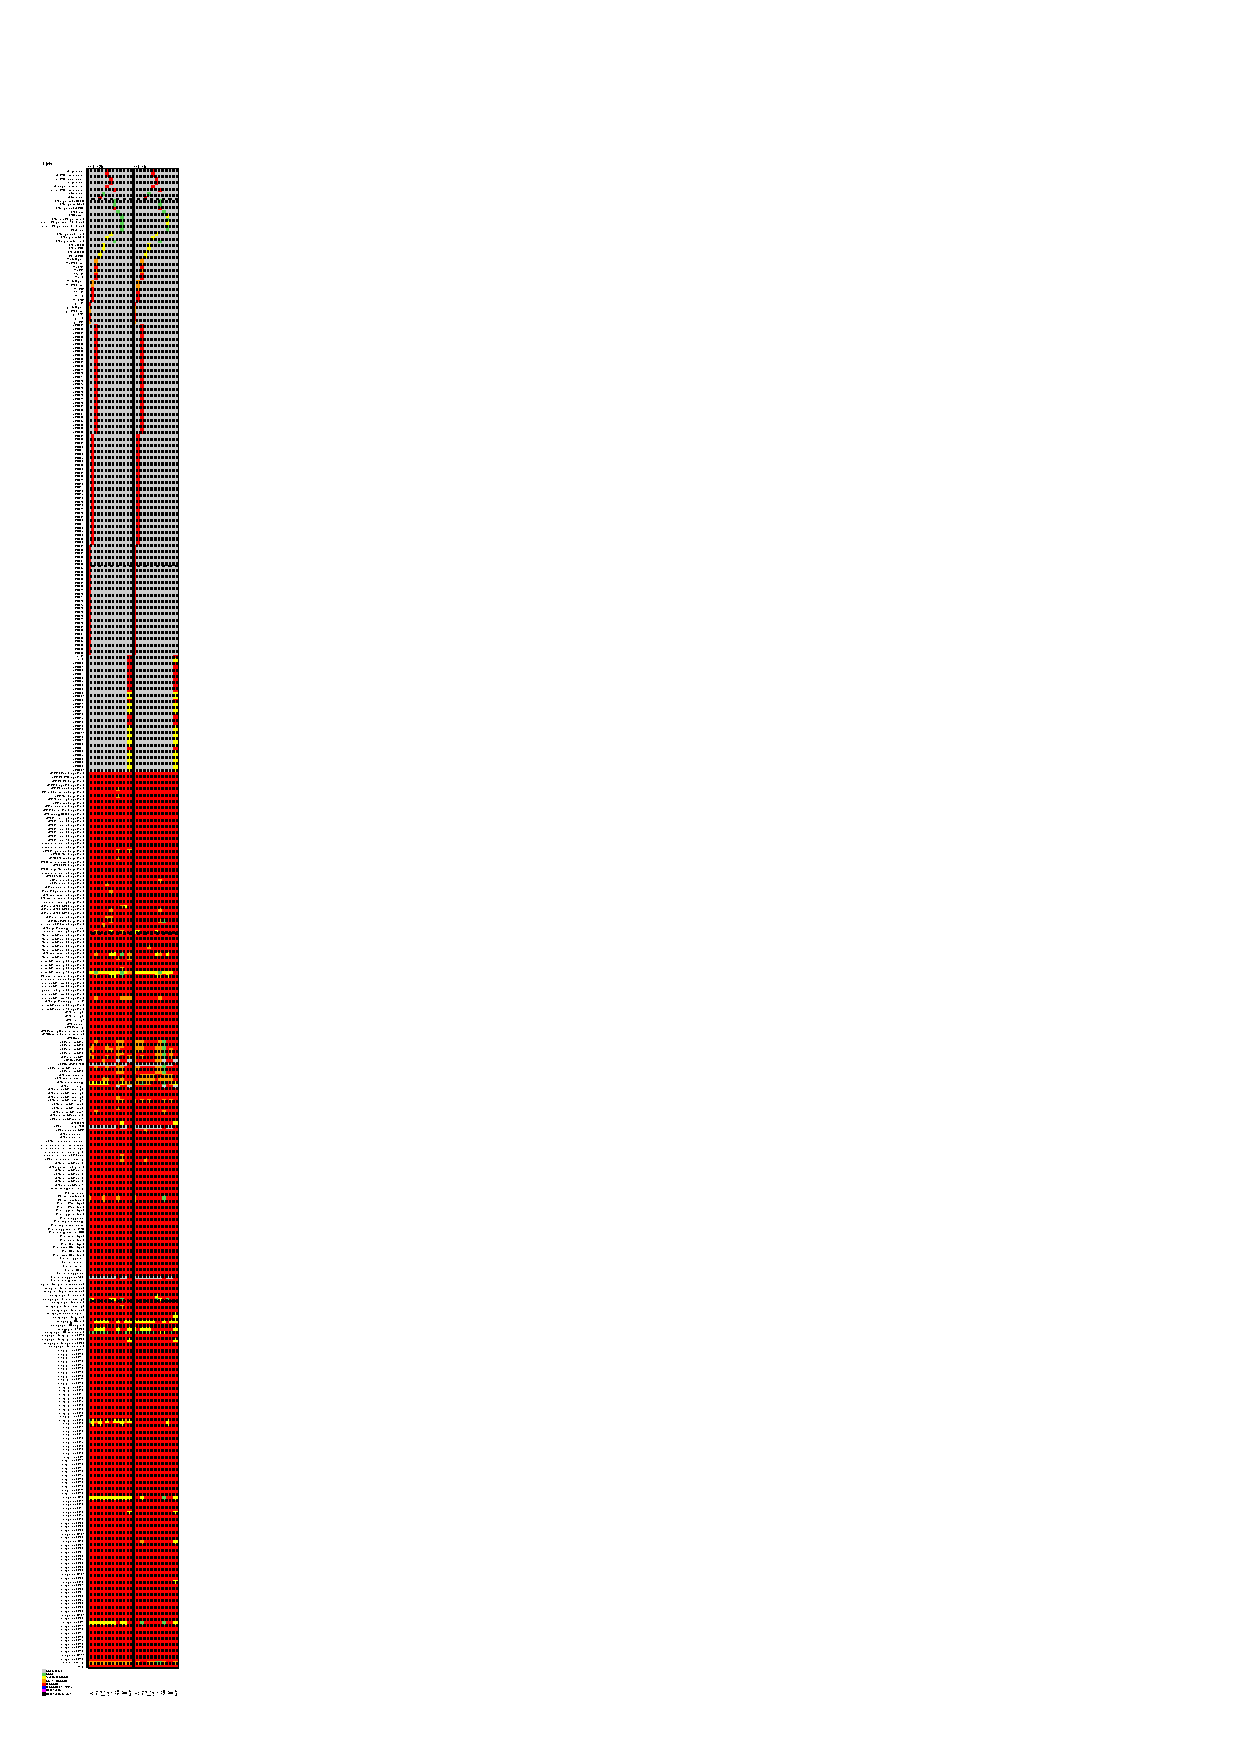
\includegraphics[keepaspectratio, scale=0.85]{images/Pruning/Pruning_Asimov_Hp3000_Contained80_DL1r_70.pdf}
  \caption{Pruned systematic uncertainties in the 3000 GeV $H^{+}$ mass Asimov fits}
  \label{fig:Pruning_Asimov_Hp3000_Contained80_DL1r_70}
\end{figure}

